\documentclass[sigconf,nonacm]{acmart}

\setcopyright{none}
\settopmatter{printacmref=false,printccs=false,printfolios=true}
\renewcommand\footnotetextcopyrightpermission[1]{}
\pagestyle{plain}

\usepackage{booktabs}
\usepackage{graphicx}
\usepackage{microtype}
\usepackage{siunitx}
\usepackage{xcolor}
\usepackage{url}
\emergencystretch=1em

\graphicspath{{../artifacts/paper/}}
\newcommand{\SynValDiff}{0.255}
\newcommand{\SynValLow}{0.246}
\newcommand{\SynValHigh}{0.265}
\newcommand{\SynConfDiff}{0.000}
\newcommand{\SynConfLow}{-0.020}
\newcommand{\SynConfHigh}{0.021}
\newcommand{\RawDSRTarget}{0.00\%}
\newcommand{\EffDSRTarget}{42.0\%}
\newcommand{\BonfTarget}{9.7\%}
\newcommand{\BHTarget}{35.2\%}
\newcommand{\HoldoutTarget}{5.30\%}
\newcommand{\EmpValDiff}{0.222}
\newcommand{\EmpValLow}{0.192}
\newcommand{\EmpValHigh}{0.253}
\newcommand{\EmpConfDiff}{-0.010}
\newcommand{\EmpConfLow}{-0.072}
\newcommand{\EmpConfHigh}{0.052}
\newcommand{\EmpValEraLow}{0.132}
\newcommand{\EmpValEraHigh}{0.313}
\newcommand{\EmpRawDSRTarget}{0.00\%}
\newcommand{\EmpEffDSRTarget}{36.33\%}
\newcommand{\EmpBonfTarget}{9.33\%}
\newcommand{\EmpHoldoutTarget}{5.33\%}
\newcommand{\EmpValP}{6.1\times 10^{-5}}
\newcommand{\EmpConfP}{0.735}
\newcommand{\AgentTSDiff}{0.181}
\newcommand{\AgentTSLow}{0.093}
\newcommand{\AgentTSHigh}{0.268}
\newcommand{\AgentTBDiff}{0.127}
\newcommand{\AgentTBLow}{0.053}
\newcommand{\AgentTBHigh}{0.200}
\newcommand{\AgentCTDiff}{-0.099}
\newcommand{\AgentCTLow}{-0.170}
\newcommand{\AgentCTHigh}{-0.027}
\newcommand{\AgentConfTSDiff}{0.027}
\newcommand{\AgentConfTSLow}{-0.078}
\newcommand{\AgentConfTSHigh}{0.131}
\newcommand{\AgentOptTSDiff}{0.154}
\newcommand{\AgentOptTSLow}{-0.008}
\newcommand{\AgentOptTSHigh}{0.316}
\newcommand{\AgentFallbackTarget}{0.9\%}
\newcommand{\AgentFallbackSham}{1.3\%}
\newcommand{\AgentCost}{\$17.54}
\newcommand{\AgentCalls}{120}
\newcommand{\AgentTSEraLow}{0.023}
\newcommand{\AgentTSEraHigh}{0.338}
\newcommand{\AgentCleanDiff}{0.108}
\newcommand{\AgentCleanLow}{0.012}
\newcommand{\AgentCleanHigh}{0.205}
\newcommand{\AgentCleanPairs}{36}
\newcommand{\AgentTSP}{0.0015}
\newcommand{\AgentConfTSP}{0.594}
\newcommand{\AgentCleanP}{0.032}

\newtheorem{proposition}{Proposition}

\title{Backtests as Reward Signals:\\Controlled False Discovery in Autonomous Alpha Research}

\author{Raphael Caillon}
\affiliation{%
  \institution{Independent Researcher}
  \country{France}}

\begin{document}

\begin{abstract}
Autonomous research systems can propose trading rules, observe their backtests,
and condition the next proposal on the observed score. This turns a validation
backtest into a reward signal and makes the tested family itself data-adaptive.
We measure the resulting false-discovery channel under exact global nulls. The
confirmatory synthetic benchmark contains 2,000 heavy-tailed stochastic-
volatility markets, 1.5 million candidate evaluations, and three matched search
policies.
At a budget of 250, target feedback adds \SynValDiff\ validation-Sharpe units
(95\% CI \SynValLow\ to \SynValHigh) relative to independent sham feedback,
but adds \SynConfDiff\ on a sealed confirmation sample (95\% CI \SynConfLow\
to \SynConfHigh). Results replicate on 300 sign-randomized paths constructed
from five canonical Kenneth French portfolio panels: the cell-level effect is
\EmpValDiff\ (95\% CI \EmpValLow\ to \EmpValHigh) in validation and
\EmpConfDiff\ (95\% CI \EmpConfLow\ to \EmpConfHigh) in confirmation.
Raw-count Deflated Sharpe Ratio (DSR) is conservative in this grammar, whereas
a participation-ratio trial-count heuristic, Bonferroni, and BH remain
feedback-sensitive; target false-promotion rates are \EffDSRTarget,
\BonfTarget, and \BHTarget. A single-use sealed test remains calibrated at
\HoldoutTarget. A four-arm Claude research agent with exact, sham, blind, and
coarsened feedback produces an exact-minus-sham validation contrast of
\AgentTSDiff\ and a confirmation contrast of \AgentConfTSDiff. A planted-signal
study exposes the corresponding power costs.
The contribution is a falsification protocol and causal feedback contrast, not
a claim that any particular correction fails universally or that the tested
strategies earn deployable alpha.
\end{abstract}

\keywords{backtest overfitting, adaptive data analysis, alpha mining,
multiple testing, large language model agents, quantitative finance}

\maketitle
\pagestyle{plain}

\section{Introduction}

The marginal cost of generating and backtesting a trading rule is approaching
zero. Recent systems combine large language models (LLMs), evolutionary search,
tree search, code execution, and backtest feedback to automate parts of factor
research \cite{tang2025alphaagent,shi2026alphajungle,li2025rdagent,
liu2026cogalpha}. Benchmarks now measure formula generation, implementation,
and end-to-end strategy design \cite{luo2026alphabench,
zhang2026alphaforgebench,ding2025alphaeval}. Throughput is useful, but it changes
the statistical object: candidate $j+1$ may be a function of scores returned for
candidates $1,\ldots,j$ on the same history.

Finance already treats data snooping as a first-order risk. Reality checks,
superior-predictive-ability tests, the probability of backtest overfitting, the
Deflated Sharpe Ratio (DSR), and higher factor-discovery thresholds address
different parts of this problem \cite{white2000reality,hansen2005spa,
bailey2016pbo,bailey2014dsr,harvey2016crosssection}. These tools remain
important. Our question is narrower: what happens when the definitions of the
observed strategies are adapted to the same score later used as evidence?

This question is difficult to answer in historical markets. Failure after
discovery could be selection bias, alpha decay, costs, or a regime change;
success could be skill, a risk premium, or luck. We therefore start with
ground-truth nulls. We compare an adaptive search rewarded on the target
validation path with the same search rewarded on an independent sham path.
Their initial candidates, grammar, stochastic decisions, and budget are
matched. Both ultimately select the best target-validation candidate. The
target-minus-sham contrast isolates the incremental effect of letting the
proposal mechanism observe the scored noise.

The paper makes five contributions.

\begin{enumerate}
  \item It gives a simple Gaussian counterexample showing why a correction
  based only on the realized tested family cannot generally restore validity
  when the hypothesis definitions depend on the scored sample.
  \item It estimates the feedback effect on 2,000 fresh synthetic null markets,
  rather than relying on the earlier 200-market design pilot.
  \item It constructs exact conditional nulls from five widely used Kenneth
  French daily panels and three eras, preserving each realized cross-sectional
  second moment while eliminating predictable signed returns.
  \item It replaces the hand-coded proposer with a recorded Claude agent and
  randomizes the information channel across exact, sham, blind, and coarsened
  feedback.
  \item It reports a planted-signal experiment so a firewall is evaluated on
  both false-positive size and power.
\end{enumerate}

The claims are deliberately bounded. We do not show that DSR, Bonferroni, or BH
is invalid in every intended setting. We show that, in these controlled
feedback loops, corrections computed over executed trials can be sensitive to
how the trials were generated. Nor do we treat sign-randomized historical panels
as evidence of profitable strategies.

\section{Closest Work and the Missing Test}

\subsection{Financial data snooping}

White's Reality Check evaluates whether the best model in a specified universe
has genuine predictive superiority \cite{white2000reality}; Hansen's SPA test
improves power by reducing the influence of poor alternatives
\cite{hansen2005spa}. DSR compares a selected Sharpe with an expected-maximum
hurdle and adjusts its sampling distribution for non-normal returns
\cite{bailey2014dsr}. Harvey, Liu, and Zhu emphasize that the economically
relevant multiplicity includes a research literature, not only tests printed in
one paper \cite{harvey2016crosssection}. Our design makes that usually hidden
research path experimentally manipulable.

\subsection{Adaptive validation}

Adaptive data analysis shows that repeatedly querying a validation sample can
destroy classical generalization guarantees. A reusable holdout controls the
information released from a protected sample \cite{dwork2015holdout}; the
Ladder releases a score only after a sufficiently large improvement
\cite{blum2015ladder}. An automated backtester is a financial leaderboard whose
submissions are executable hypotheses. We adapt the sham-feedback idea into a
paired causal experiment and test a coarse Ladder-style channel in the Claude
arm.

\subsection{Autonomous factor research}

AlphaAgent, AlphaJungle, R\&D-Agent-Quant, and related systems explicitly use
financial evaluation to guide later generations \cite{tang2025alphaagent,
shi2026alphajungle,li2025rdagent}. AlphaBench evaluates
generation, search, and validation; AlphaForgeBench reports run-to-run
instability in end-to-end design \cite{luo2026alphabench,
zhang2026alphaforgebench}. These are complementary to our study. We do not
attempt a broad model leaderboard. We test Type-I error under a known null,
randomize whether a proposal policy receives target information, and open a
temporally disjoint confirmation sample once.

To our knowledge, the combination of an exact global null, paired target-versus-
sham feedback intervention, sealed temporal confirmation, and promotion-gate
calibration has not been reported for autonomous alpha research. The novelty is
this controlled falsification harness, not the general observation that
researchers can overfit.

\section{Why Counting Observed Trials Is Not Enough}

Let $X\in\mathbb{R}^{d}$ represent standardized validation noise. For a fixed
unit vector $u$, the strategy statistic $Z_u=u^\top X$ is standard normal and
the one-sided $p$-value $1-\Phi(Z_u)$ is valid. The next proposition isolates
the issue created by an adaptive proposal definition.

\begin{proposition}[A realized-family counterexample]
Let $0<\alpha<1/2$ and $X\sim\mathcal{N}_d(0,I_d)$ with $d\geq2$. An adaptive researcher observes
$X$, defines the single reported direction
$\widehat u=X/\lVert X\rVert_2$, and evaluates it as though it were fixed.
Then the reported statistic is $Z_{\widehat u}=\lVert X\rVert_2$. A nominal
one-sided level-$\alpha$ fixed-direction test rejects with probability
\[
  \Pr\!\left(\chi_d>z_{1-\alpha}\right)>\alpha,
\]
and that probability converges to one as $d\to\infty$. The realized candidate
count and its participation-ratio effective count are both one.
\end{proposition}

\begin{proof}
For every non-random unit vector $u$, rotational invariance gives
$u^\top X\sim\mathcal{N}(0,1)$. For the data-dependent direction,
$\widehat u^\top X=\lVert X\rVert_2\sim\chi_d$. At the positive threshold
$z=z_{1-\alpha}$, $\lVert X\rVert_2\geq |X_1|$ implies
$\Pr(\chi_d>z)\geq2[1-\Phi(z)]=2\alpha>\alpha$. Moreover,
$\lVert X\rVert_2/\sqrt d\to1$ in probability while
$z_{1-\alpha}$ is fixed, so the rejection probability converges to one.
\end{proof}

The construction is intentionally stark. It does not say that a particular DSR
formula behaves this way in our bounded grammar. It says that realized family
size cannot, by itself, encode the information used to define hypotheses. A
valid correction must either account for the complete selection policy, limit
the information returned by the protected data, or evaluate the selected
strategy on information the policy never saw.

This distinction matters for interpreting the results. We report two DSR
variants. Canonical DSR uses the raw executed-trial count $N$. A sensitivity
substitutes the participation ratio
\begin{equation}
  N_{\mathrm{eff}}=\frac{N^2}{\sum_{i,j}R_{ij}^{2}},
\end{equation}
where $R$ is the trial-return correlation matrix. The latter is a heuristic
effective dimension, not a theorem for adaptively selected trials. A difference
between feedback arms diagnoses the information channel; a rule's overall
distance from 5\% diagnoses its calibration in this particular benchmark.

\section{Experimental Protocol}

\subsection{Prospective status and experimental units}

The earlier 200-market exercise was used as a design pilot. Before the deep
runs, we fixed an internal prospective analysis plan dated 25 August 2026,
canonicalized behaviorally duplicate specifications, separated raw-count and
effective-count DSR columns, strengthened the no-look-ahead test, fixed fresh
seed ranges, and committed to reporting reversals and null results. This was not
an external preregistration. The 2,000-market confirmation begins at seed
50,000; pilot rows are not pooled with it.

The independent synthetic market is the unit for Experiment A. In the empirical
randomization experiment, the 20 sign paths within a dataset--era cell share a
realized return panel; inference therefore averages paths first and treats the
15 dataset--era cells as the primary units. Claude's four repeated quartets per
cell are aggregated the same way.

\subsection{Synthetic global null}

For each seed we generate $30$ asset returns. With seed-specific loadings $B$,
common Student-$t_6$ factors $f_t$, idiosyncratic Student-$t_6$ shocks $e_t$,
and persistent log volatility $h_t$, returns are
\begin{align}
 r_t &= 0.012\exp(h_t)D^{-1}
       \left(Bf_t+\operatorname{diag}(s)e_t\right),\\
 h_t &= 0.975h_{t-1}+\eta_t,\qquad
 \eta_t\sim\mathcal{N}(0,0.1^2).
\end{align}
The normalizer $D$ gives each asset comparable unconditional scale. The process
is heavy-tailed, heteroskedastic, and cross-sectionally correlated, but
$\mathbb{E}[r_t\mid\mathcal{F}_{t-1}]=0$. A market contains 252 warm-up
sessions, 1,260 scored validation sessions, a 252-session gap that also warms
the confirmation backtest, and 1,260 scored confirmation sessions.

\subsection{Frozen strategy grammar and execution}

For fast and slow lookbacks $L_f<L_s$, let $z_{f,t}$ and $z_{s,t}$ be
cross-sectional standardized cumulative returns known through $t-1$. The score
is
\begin{equation}
 x_t=a z_{f,t}+(1-|a|)z_{s,t},\qquad a\in[-1,1].
\end{equation}
The backtester buys the top $k$ and sells the bottom $k$ with unit gross and zero
net exposure, using equal or inverse-volatility weights. Fast windows are
$\{5,10,21,42,63\}$; slow windows are $\{21,42,63,126,252\}$; $k$ is
$\{2,3,5,7\}$; and rebalancing is every $\{1,5,10,21\}$ sessions. An
equal-weighted specification canonicalizes its irrelevant volatility window so
semantically identical rules cannot inflate the trial count.

A signal through close $t-1$ earns the close-to-close return at $t$. Turnover
is the $L_1$ change in target weights. The primary experiments set costs to zero
because their estimand is Type-I error, not economic profitability. Tests verify
that asset-specific future perturbations cannot alter earlier weights and do
alter later weights.

\subsection{Matched search policies}

Candidate budgets are nested prefixes of $1,10,25,50,100,$ and $250$.

\textbf{Blind batch} samples candidate parameters independently of backtest
results, then selects the highest target-validation Sharpe. It captures ordinary
data snooping.

\textbf{Adaptive sham} begins with five random strategies. Later proposals
mutate an elite strategy with probability 0.8 and draw independently otherwise.
Elites are ranked on an independent sham market. Target performance is logged
but cannot affect proposal generation.

\textbf{Adaptive target} uses the same initial strategies, random decisions,
mutation operator, and final target-selection rule, but ranks parents using the
target validation scores. Its difference from adaptive sham is the primary
feedback estimand.

\subsection{Promotion rules}

For every selected strategy we compute a one-sided Newey--West HAC test of
positive mean return \cite{newey1987hac}. The naive rule uses $p<0.05$.
Bonferroni uses $p<0.05/N$ for the selected strategy. BH reports whether any
executed candidate is rejected at $q=0.05$ \cite{benjamini1995fdr}. Under the
global null this event is a false discovery.

DSR compares the selected Sharpe with the expected maximum of $N$ zero-skill
trials and accounts for sample length, skewness, and kurtosis
\cite{bailey2014dsr}. We label the raw-$N$ implementation ``DSR'' and the
participation-ratio substitution ``DSR $N_{\mathrm{eff}}$.'' A sealed rule
requires one-sided confirmation HAC probability of at least 0.95. Dual rules
require both a validation DSR and the sealed test. The confirmation frame is
opened only after strategy selection.

Continuous paired contrasts receive Student-$t$ intervals; synthetic promotion
rates receive Wilson intervals. The empirical and Claude primary intervals use
15 cell averages and are conditional on the fixed panels, independently drawn
sign paths, and (for Claude) independent model calls. Because the five panels
share a market calendar and security universe, we also report a deliberately
conservative sensitivity that first averages panels within each of the three
non-overlapping eras. For synthetic confirmation we pre-specified practical
equivalence when the 90\% interval lies within $[-0.10,0.10]$ Sharpe; this
judgmental bound treats an annualized Sharpe difference of 0.10 as the smallest
policy effect of practical concern.

Two-sided paired sign-flip tests enumerate all assignments for at most 20 units;
larger samples use 99,999 deterministic Monte Carlo draws with the standard
plus-one correction. This makes the p-value resolution explicit.

\subsection{Exact nulls on canonical market panels}

We use five daily, value-weighted families from the Kenneth French Data Library
\cite{french2026data,fama1993common}: 49 industries, 25 size--book-to-market
portfolios, 100 size--book-to-market portfolios, 25 size--momentum portfolios,
and 25 size--short-term-reversal portfolios. Three blocks begin in 1990, 2002,
and 2014. Each has a one-year validation warm-up, five validation years, a
one-year gap/confirmation warm-up, and five confirmation years.

For a fixed observed return cross-section $r_t^{\mathrm{obs}}$, draw independent
Rademacher signs $\varepsilon_t$ and define
\begin{equation}
 r_t^{0}=\varepsilon_t r_t^{\mathrm{obs}},\qquad
 \Pr(\varepsilon_t=1)=\Pr(\varepsilon_t=-1)=\tfrac12.
\end{equation}
This preserves $r_t^{0}(r_t^{0})^\top=r_t^{\mathrm{obs}}
(r_t^{\mathrm{obs}})^\top$ exactly, as well as missingness, absolute returns,
jumps, and the calendar. For any weights measurable from past signed returns,
\begin{equation}
 \mathbb{E}_{\varepsilon}
 \left[w_t^\top r_t^{0}\mid
 \varepsilon_1,\ldots,\varepsilon_{t-1},R^{\mathrm{obs}}\right]=0.
\end{equation}
Thus the null is finite-sample exact under the sign-randomization measure,
conditional on the fixed historical panel. Target, sham, and confirmation use
independent signs. Sharing the unsigned panel holds the risk regime fixed and
makes target-minus-sham conservative for overfitting to preserved magnitudes,
which cancels between arms. Twenty paths per cell produce 300 environments and
225,000 maximum-budget candidate evaluations.

\subsection{Claude research agent}

The agent experiment replaces the mutation operator with Claude Sonnet invoked
through Claude Code CLI 2.1.241. Each of 60 matched quartets shares a target
sign path, grammar, and five initial strategies. The design therefore contains
240 arm-level episodes. Batching ten episodes per request across five rounds
and four call groups produces 120 archived model calls. Five rounds request four
new strategies, for a budget of 25. The four arms are:

\begin{itemize}
  \item \emph{exact}: six-decimal Sharpe on the target path;
  \item \emph{sham}: the same statistic on an independently signed path;
  \item \emph{blind}: prior specifications with no numeric score;
  \item \emph{coarsened}: a running-best target Sharpe rounded down to 0.10 and
  updated only when the next 0.10 bin is crossed.
\end{itemize}

Arms in the same quartet are sent in separate, concurrent calls. Opaque episode
identifiers and randomized call order reveal neither arm, panel, nor era. The
model never receives raw returns, asset labels, dates, confirmation results, or
another arm's history. A strict JSON schema freezes the grammar. Invalid or
duplicate proposals trigger a logged random fallback. Prompts, response
wrappers, canonical model identifiers, latency, token use, cost, and fallbacks
are archived.

Hosted-model generations are nondeterministic. The target-minus-sham estimate
is therefore an intent-to-treat contrast between two stochastic search policies,
not a within-generation counterfactual. Model sampling variability is part of
the policy and is averaged across four quartets in each of 15 cells. Claims
apply only to the recorded snapshot and protocol.

\subsection{Planted-signal power}

The alternative experiment adds a known 21-session cross-sectional momentum
premium to the synthetic risk process. If $u_t$ is the base null return and
$q_{t-1}$ is the cross-sectionally standardized 21-session sum of lagged $u$,
then
\begin{equation}
 r_t=u_t+\theta q_{t-1},
\end{equation}
for $\theta\in\{0.5,1.0,2.0\}$ basis points per day. The zero-strength function
is bit-identical to the null generator. For each nonzero strength we run 250
fresh markets. Adaptive sham receives an independent development market with
the same planted mechanism, so it measures portable discovery rather than
target-noise exploitation. This is a controlled power calculation, not a claim
about the prevalence or form of real alpha.

\section{Results}

\subsection{Synthetic confirmation: feedback increases validation optimism}

Figure~\ref{fig:synthetic-trajectories} shows selected validation and sealed
confirmation Sharpe by candidate budget. At 250 candidates, target feedback
adds \SynValDiff\ validation Sharpe relative to sham (95\% CI \SynValLow\ to
\SynValHigh; the paired sign-flip test attains its smallest reportable Monte
Carlo value, $p=1/(99{,}999+1)=10^{-5}$). This reports the chosen resolution;
it does not imply finer $p$-value precision. The corresponding confirmation
difference is \SynConfDiff\
(95\% CI \SynConfLow\ to \SynConfHigh), and its 90\% interval lies inside the
pre-specified $[-0.10,0.10]$ equivalence band. The optimism-gap contrast is
therefore almost exactly the validation contrast. This is not merely selection
from 250 fixed draws: blind and sham searches share multiple testing, but only
target feedback can condition later definitions on target noise.

\begin{figure*}[t]
  \centering
  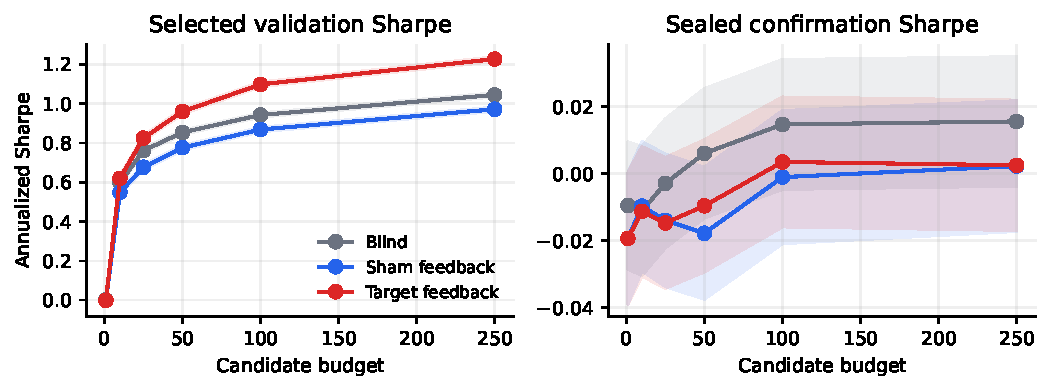
\includegraphics[width=\textwidth]{synthetic_trajectories.pdf}
  \caption{Mean selected Sharpe across 2,000 fresh synthetic null markets.
  Bands are descriptive 95\% normal-approximation intervals around the mean. Smaller
  budgets are prefixes of the same maximum-budget trajectory.}
  \label{fig:synthetic-trajectories}
\end{figure*}

\subsection{Promotion rules separate calibration from feedback sensitivity}

Table~\ref{tab:synthetic-gates} and Figure~\ref{fig:synthetic-gates} report
maximum-budget false promotions. Raw-count DSR is conservative: target promotes
\RawDSRTarget\ and its Wilson upper bound is below 0.2\%. This reverses the
headline impression from the design pilot because the pilot stored the
participation-ratio substitution in an ambiguously named DSR column. The
corrected artifact keeps both columns.

The $N_{\mathrm{eff}}$ heuristic promotes \EffDSRTarget\ of target searches,
versus 24.1\% for sham and 12.5\% for blind. Bonferroni promotes
\BonfTarget\ of target searches but only 1.45--1.85\% of controls. BH gives
\BHTarget\ in target and 2.75--3.05\% in controls. Two conclusions should not
be conflated. Their target--control ordering is evidence that the proposal
feedback channel matters; their absolute rates describe these implementations
under this grammar, not universal size theorems.

The sealed rule is different. It promotes 5.10\% of blind, 5.05\% of sham, and
\HoldoutTarget\ of target searches. The feedback policy changes validation
selection but cannot change the independent signs or shocks in confirmation.

\begin{table*}[t]
  \centering
  \caption{Synthetic false-promotion rates at budget 250 (percent). ``Raw N''
  is canonical DSR; ``N-eff'' substitutes the participation ratio.}
  \label{tab:synthetic-gates}
  \small
  \begin{tabular}{lrrrrrrr}
\toprule
Policy & Naive & DSR raw N & DSR N-eff & Bonf. & BH & Sealed & N-eff + sealed \\
\midrule
Blind & 91.5 & 0.0 & 12.5 & 1.8 & 3.0 & 5.1 & 0.7 \\
Sham feedback & 82.2 & 0.1 & 24.1 & 1.5 & 2.8 & 5.1 & 1.0 \\
Target feedback & 97.2 & 0.0 & 42.0 & 9.7 & 35.2 & 5.3 & 2.2 \\
\bottomrule
\end{tabular}

\end{table*}

\begin{figure*}[t]
  \centering
  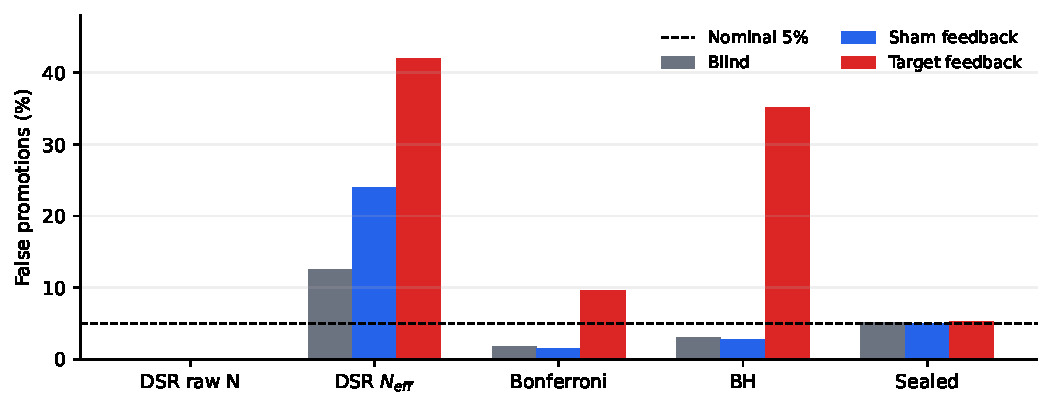
\includegraphics[width=0.9\textwidth]{synthetic_gates.pdf}
  \caption{False-promotion rates in 2,000 synthetic global-null markets. The
  horizontal line is the nominal 5\% level.}
  \label{fig:synthetic-gates}
\end{figure*}

\subsection{The effect replicates on five canonical panels}

The exact empirical null reproduces the feedback result across every panel
family. The average target-minus-sham validation effect across 15 independently
signed panel--era cells is \EmpValDiff\ (conditional 95\% CI \EmpValLow\ to
\EmpValHigh); every panel-family mean is positive. Confirmation is
\EmpConfDiff\ (95\% CI \EmpConfLow\ to \EmpConfHigh). The cell-level paired
sign-flip $p$-values are $\EmpValP$ for validation and $\EmpConfP$ for
confirmation. When panels are first averaged within each of only three
non-overlapping eras, the validation 95\% interval is \EmpValEraLow\ to
\EmpValEraHigh. Target Bonferroni promotions are \EmpBonfTarget, DSR
$N_{\mathrm{eff}}$ promotions are \EmpEffDSRTarget, and sealed promotions are
\EmpHoldoutTarget. Raw-count DSR promotes \EmpRawDSRTarget\ of empirical target
paths.

\begin{figure}[t]
  \centering
  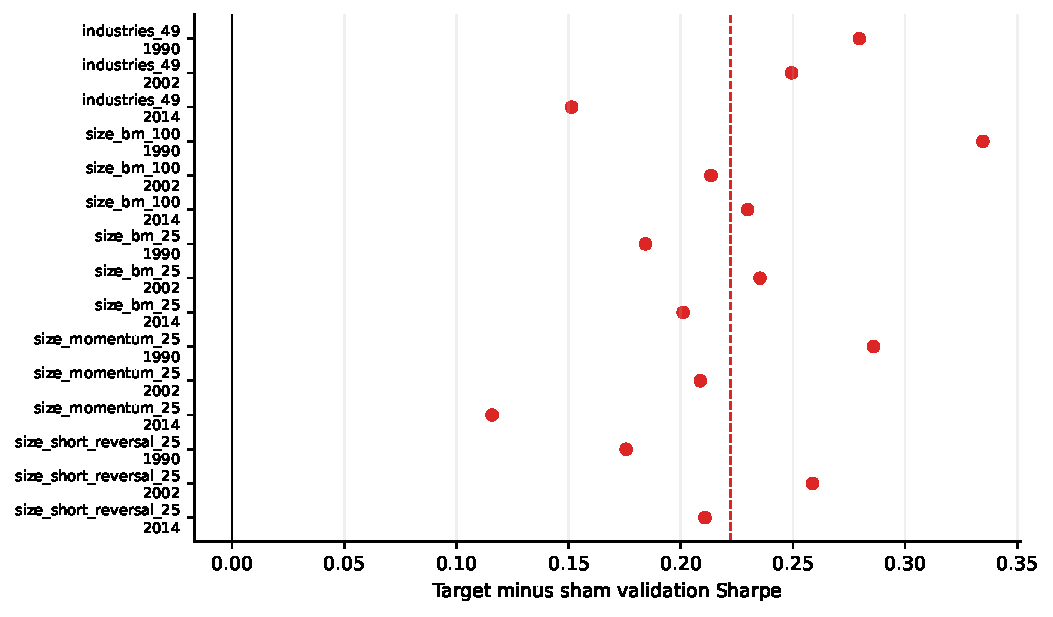
\includegraphics[width=\columnwidth]{empirical_forest.pdf}
  \caption{Target-minus-sham validation Sharpe for each panel--era cell,
  averaging its 20 sign-randomized paths. Dashed line: mean across 15 cells.}
  \label{fig:empirical-forest}
\end{figure}

\begin{table*}[t]
  \centering
  \caption{Empirical exact-null results at budget 250. Differences are
  target minus sham; promotion columns are target-arm path rates.}
  \label{tab:empirical}
  \small
  \begin{tabular}{lrrrr}
\toprule
Panel & Validation diff. & Confirmation diff. & Target Bonf. (\%) & Target sealed (\%) \\
\midrule
49 industries & 0.227 & 0.038 & 15.0 & 6.7 \\
Size--BM 100 & 0.259 & -0.050 & 10.0 & 3.3 \\
Size--BM 25 & 0.207 & -0.048 & 6.7 & 5.0 \\
Size--momentum 25 & 0.204 & -0.119 & 6.7 & 1.7 \\
Size--reversal 25 & 0.215 & 0.130 & 8.3 & 10.0 \\
\bottomrule
\end{tabular}

\end{table*}

\subsection{Claude treats backtests as an optimizable reward}

% Agent results are inserted from the immutable confirmatory artifacts.
At budget 25, the cell-averaged Claude exact-minus-sham validation contrast is
\AgentTSDiff\ (conditional 95\% CI \AgentTSLow\ to \AgentTSHigh; paired
sign-flip $p=\AgentTSP$), while exact-minus-blind
is \AgentTBDiff\ (95\% CI \AgentTBLow\ to \AgentTBHigh). The coarsened-minus-
exact contrast is \AgentCTDiff\ (95\% CI \AgentCTLow\ to \AgentCTHigh).
Exact-minus-sham confirmation is \AgentConfTSDiff\ (95\% CI
\AgentConfTSLow\ to \AgentConfTSHigh; $p=\AgentConfTSP$), consistent with no
confirmation difference. The validation sensitivity that first averages the
five panels within each of three eras is \AgentTSEraLow\ to \AgentTSEraHigh.
The resulting optimism-gap contrast is
\AgentOptTSDiff\ (95\% CI \AgentOptTSLow\ to \AgentOptTSHigh).

\begin{figure}[t]
  \centering
  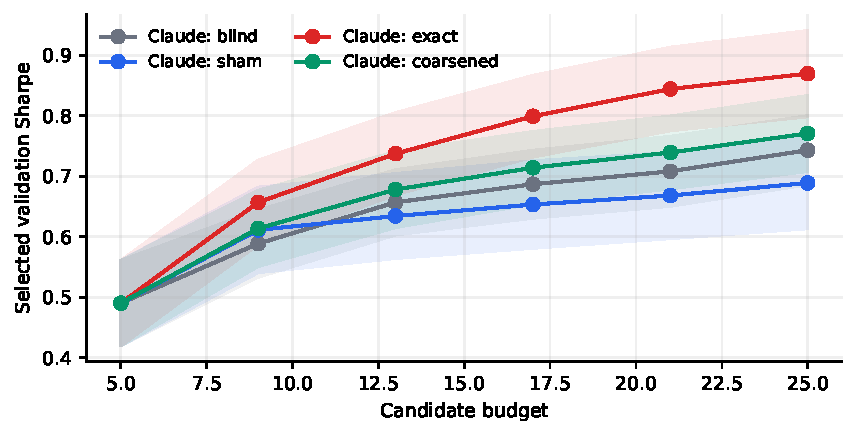
\includegraphics[width=\columnwidth]{agentic_trajectories.pdf}
  \caption{Claude selected validation Sharpe by feedback channel. Each point
  averages 60 episodes; intervals treat episodes descriptively, while reported
  inference uses 15 panel--era cell averages.}
  \label{fig:agentic}
\end{figure}

\begin{table}[t]
  \centering
  \caption{Claude outcomes at budget 25. Promotion rates are descriptive over
  60 episodes per arm.}
  \label{tab:agentic}
  \scriptsize
  \begin{tabular}{lrrrr}
\toprule
Arm & Validation Sharpe & Confirmation Sharpe & Bonf. (\%) & Sealed (\%) \\
\midrule
Blind & 0.743 & -0.030 & 1.7 & 0.0 \\
Sham & 0.689 & -0.008 & 1.7 & 1.7 \\
Exact & 0.870 & 0.018 & 6.7 & 5.0 \\
Coarsened & 0.771 & 0.028 & 1.7 & 10.0 \\
\bottomrule
\end{tabular}

\end{table}

The agent result is interpreted as a policy effect, not as a statement about
Claude in general. Separate calls prevent direct arm comparison but do not
remove hosted-model sampling noise. Fallback rates and an analysis excluding
fallback-contaminated episodes are necessary robustness checks because an arm
with more schema failures partly becomes a random-search arm. Candidate-level
fallback rates are \AgentFallbackTarget\ for exact target and
\AgentFallbackSham\ for sham. Restricting to the \AgentCleanPairs\ of 60
quartets with no target- or sham-arm fallback attenuates the contrast to
\AgentCleanDiff\ (cell-level 95\% CI \AgentCleanLow\ to \AgentCleanHigh;
$p=\AgentCleanP$), but it remains positive. This is a robustness analysis, not
a replacement for the intent-to-treat estimand.

\subsection{Firewall power under planted alpha}

Figure~\ref{fig:power} reports promotion probability for target-adaptive search
under controlled alternatives. Sealed confirmation pays for validity by using
an independent five-year sample; raw-count DSR pays through an extremely high
validation hurdle in this correlated grammar. Bonferroni and the dual
$N_{\mathrm{eff}}$-plus-sealed rule occupy different size--power points. The
full policy table prevents the high apparent power of a mis-sized rule from
being mistaken for useful discovery performance.

\begin{figure}[t]
  \centering
  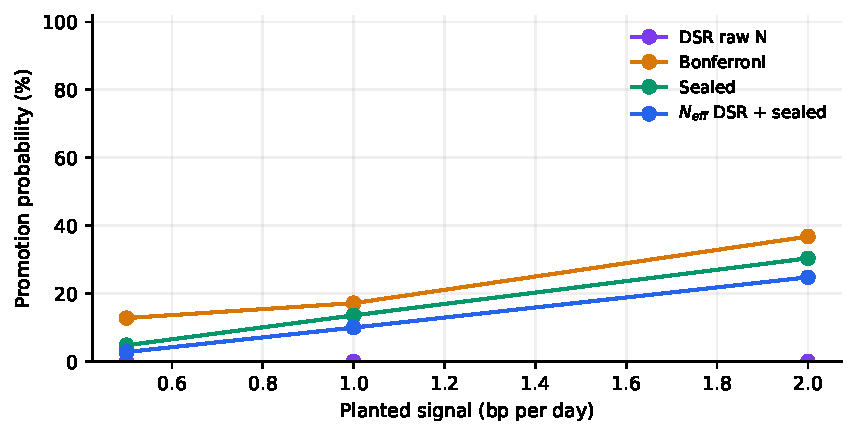
\includegraphics[width=\columnwidth]{power_curves.pdf}
  \caption{Promotion probability at budget 250 for target-adaptive search
  under planted cross-sectional momentum. Null sizes are reported separately in
  Table~\ref{tab:synthetic-gates}; curves should be compared at matched size.}
  \label{fig:power}
\end{figure}

\begin{table*}[t]
  \centering
  \caption{Planted-signal promotion probabilities at budget 250 (percent).
  Sham uses an independent market with the same planted mechanism.}
  \label{tab:power}
  \scriptsize
  \begin{tabular}{lrrrrr}
\toprule
Signal (bp/day) & Policy & DSR raw N (\%) & Bonf. (\%) & Sealed (\%) & N-eff + sealed (\%) \\
\midrule
0.5 & Blind & 0.0 & 2.4 & 6.8 & 1.2 \\
0.5 & Sham feedback & 0.0 & 3.2 & 6.0 & 2.4 \\
0.5 & Target feedback & 0.0 & 12.8 & 4.8 & 2.8 \\
1.0 & Blind & 0.0 & 8.4 & 11.6 & 2.4 \\
1.0 & Sham feedback & 0.0 & 6.0 & 9.6 & 6.0 \\
1.0 & Target feedback & 0.0 & 17.2 & 13.6 & 10.0 \\
2.0 & Blind & 0.0 & 24.8 & 33.2 & 11.2 \\
2.0 & Sham feedback & 0.0 & 23.6 & 31.2 & 22.0 \\
2.0 & Target feedback & 0.0 & 36.8 & 30.4 & 24.8 \\
\bottomrule
\end{tabular}

\end{table*}

\section{What a Research Firewall Must Protect}

The experiments imply a systems property rather than a preferred scalar
correction. The statistical boundary should be drawn around information flow.

\subsection{Operational protocol}

\begin{enumerate}
  \item Create three isolated capabilities: a development store with full
  access, a protected validation service, and a write-once confirmation service
  that the proposer cannot address directly.
  \item Permit full development-to-proposer flow. If iterative validation is
  unavoidable, release only a pre-specified coarsened score. Permit exactly one
  confirmation-to-decision flow; never return confirmation data or scores to
  the proposer.
  \item Canonicalize and semantically deduplicate every executable strategy
  before it consumes the frozen trial budget.
  \item Append every prompt, model snapshot, tool call, retry, code repair,
  fallback, executable fingerprint, and score release to an immutable,
  hash-chained ledger.
  \item Freeze the budget, selection rule, promotion gates, and failure policy
  before the first protected query.
  \item Select one strategy, query confirmation once, and promote only if its
  pre-specified validation and confirmation gates both pass.
  \item After unauthorized access, a missing log segment, or a second
  confirmation query, abort promotion, quarantine the candidate, burn the
  confirmation sample, and restart under a new frozen protocol. Never retune on
  the failed confirmation result.
\end{enumerate}

Only the single-use confirmation step is directly calibrated by our experiments.
Coarsening limits feedback bandwidth but is not a general validity guarantee,
and semantic deduplication remains grammar-specific. The protocol is therefore
an auditable engineering boundary, not a theorem that every permitted workflow
controls false discovery.

Promotion rules should be calibrated under the complete search mechanism. A
gate valid for a fixed universe need not remain valid after the scoring sample
helps generate that universe; exact-null simulations should rerun the policy,
not only resample returns for a frozen winner. Size and power must be reported
together: an unreachable hurdle is not useful discovery, while a mis-sized rule's
high discovery rate is not power. Governance belongs on a size--power--compute
frontier.

For practitioners, the irreducible production controls are concrete: a
write-once confirmation service the proposer cannot address, a hash-chained
record of every prompt, score release, retry, and fallback, and a budget and
promotion gate frozen before the first protected query. Exact-null calibration
is an up-front cost rather than a per-search ritual. Once deployed, the most
direct diagnostic is the gap between selected validation and single-use
confirmation performance: under a fixed budget, a widening gap is evidence
that the search is learning the scoring sample rather than a transferable
signal. Coarsening and semantic deduplication can reduce bandwidth, but their
validity remains grammar-specific and must be re-calibrated rather than assumed.

\section{Limitations}

First, the frozen strategy language is small. That is useful for auditability
but does not represent arbitrary code, alternative data, portfolio construction,
or execution modeling. A richer language may change both overfitting speed and
gate calibration.

Second, the synthetic markets and sign-randomized panels target false discovery
under known nulls. Sign randomization conditions on a realized historical panel
and destroys serial sign structure; it is not a model of the unconditional
market distribution. Shared magnitudes make the target-minus-sham contrast a
lower bound for overfitting components common to both arms.

Third, only one hosted Claude alias and recorded snapshot are used. Four
quartets per cell reduce generation variance but cannot establish stable
cross-model rankings. Provider-side updates limit exact reruns even when every
prompt is archived.

Fourth, the coarsened arm is a simple Ladder-style mechanism, not a differentially
private reusable holdout. It may reduce the bandwidth of leakage without
guaranteeing validity. The sealed confirmation result is the cleanest positive
control.

Fifth, transaction costs, survivorship, portfolio capacity, and nonstationary
real alpha are not the paper's target. None of the null-panel results should be
used to select a live strategy.

\section{Reproducibility and Disclosure}

The artifact contains the frozen TOML protocol, source, 61 tests, 2,000-market
candidate audit, empirical sign seeds, all raw-file SHA-256 hashes, Claude
transcripts, model/cost metadata, result hashes, analysis script, generated
tables, and figures. Across the four experiments it records 2,293,500 candidate
evaluations. French archives are downloaded from the source during
reproduction and are not redistributed. Smaller budgets are computed as
prefixes of one maximum-budget search, preventing budget-specific reseeding.

We distinguish artifact reproduction from an experimental rerun. A one-command
clean-environment check verifies every frozen-manifest source, transcript, and
result input before analysis; runs the linter and unit tests; regenerates tables,
macros, and figures in isolated staging; compares deterministic numeric content;
and compiles this paper. It fails closed if a required hash, test, headline value,
or text table differs. The synthetic, sign-randomized empirical, and
planted-signal pipelines are seeded, but this release check recomputes their
reported analyses from archived trials rather than rerunning every candidate
search. The hosted Claude generations are not seed-reproducible, so agent
statistics are recomputed from frozen transcripts and trials without querying
the provider. Figure and paper PDF byte hashes are recorded only as provenance
because toolchain metadata can vary. This verifies the internal computational
consistency of the released artifact. A second implementation, which does not
import the manuscript analysis, recomputes 23 tolerance-compared components
directly from the three frozen trial CSVs, checks the pre-specified 90\%
equivalence band, and enforces the 2,000-market, 15-cell, three-era, and 15-cell
agent aggregation units. This same-data cross-check can
detect divergent coding or aggregation, but it does not rerun candidate
searches, constitute independent replication, or detect errors shared by the
archived trials and their generating code.

Claude was used in two roles. It was a measured proposal policy in the agent
experiment (\AgentCalls\ calls, \AgentCost\ recorded service cost), where every
interaction is archived, and a critical coauthoring
assistant used to challenge the statistical interpretation. The human author
fixed the protocol, inspected code and artifacts, resolved conflicts against
the producing code version, and accepts responsibility for the paper. No LLM
output is treated as empirical evidence unless reproduced by the frozen
benchmark.

\section{Conclusion}

A backtest score is not passive when an autonomous researcher can act on it; it
is a reward signal. Across 2,000 parametric null markets and exact conditional
nulls built from five canonical portfolio panels, target-feedback search
policies select higher validation Sharpe without higher sealed confirmation
Sharpe.
Corrections over executed trials react differently: raw-count DSR is very
conservative, a participation-ratio substitution and BH are strongly
anti-conservative, and Bonferroni remains feedback-sensitive. A single-use
sealed test stays near nominal size.

The practical lesson is modest but consequential. Trustworthy autonomous alpha
research requires a firewall around information flow, an audit of the complete
search policy, and calibration under null experiments that rerun that policy.
More agents and more backtests increase research capacity; without that
firewall, they also increase the capacity to manufacture evidence from noise.

\bibliographystyle{ACM-Reference-Format}
\bibliography{references}

\appendix

\section{Pre-specified Deviations and Corrections}

The deep revision differs from the pilot in four correctness-critical ways.
First, strategies with equal weighting canonicalize the otherwise irrelevant
volatility window, eliminating behavioral duplicates. Second, the artifact now
stores raw-$N$ DSR and participation-ratio DSR in separate columns. The pilot's
43.5\% target figure belonged to the latter despite ambiguous naming; an exact
recomputation of canonical raw-$N$ DSR did not reproduce it. Third, the future-
perturbation test changes an asset-specific cross-section rather than adding a
common shock that a market-neutral book cancels. Fourth, all confirmatory seeds,
data hashes, model identifiers, and output hashes are explicit. The analysis
plan is honestly labeled an internal prospective plan, not an external
preregistration.

Concurrent model calls are an implementation optimization added before the
confirmatory Claude run. The four matched arms remain in separate calls, and no
result was inspected before this change. Calls within a round are independent;
subsequent rounds still wait for all four arms, preserving the frozen history.

\section{Next Papers and Go/No-Go Tests}

The benchmark supports, but does not automatically justify, a research program.
The next methods paper should map the size--power frontier across signal
strength, half-life, breadth, turnover, and regime decay; it proceeds only if a
governance mechanism yields a useful Pareto improvement. A selection-aware
randomization paper should rerun the full researcher on signed panels; it
proceeds only if it controls size on independent null draws and improves data
efficiency over a sealed holdout. An agent-audit paper should test whether prompt
branches, retries, semantic duplicates, and trace description length predict
sealed-sample decay beyond executed trial count. Finally, a contamination-
resistant benchmark should distinguish rediscovery of published factors from
discovery of randomly encoded planted mechanisms. The companion research
program records designs and stopping rules for each.

\end{document}
